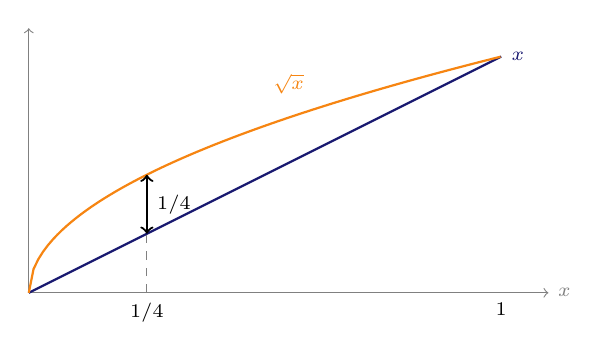
\begin{tikzpicture}[x=6cm,y=3cm,every node/.style={font=\scriptsize}]
\draw[->,gray] (0,0)--(1.1,0) node[right] {$x$};
\draw[->,gray] (0,0)--(0,1.12);
\draw[MidnightBlue,thick] (0,0)--(1,1) node[right] {$x$};
\draw[BurntOrange,thick,domain=0:1,samples=100] plot (\x,{sqrt(\x)});
\node[BurntOrange,above] at (.55,.8) {$\sqrt x$};
\draw[<->,thick] (.25,.25)--node[right] {$1/4$}(.25,.5);
\draw[gray,dashed] (.25,0)--(.25,.25);
\node[below] at (.25,0) {$1/4$};\node[below] at (1,0) {$1$};
\end{tikzpicture}
